
\section{\tool Design}
\label{sec:design}
\begin{figure*}[t]    
\centering  
\resizebox{\linewidth}{!}{%
\begin{tikzpicture}[    
    node distance=2.5cm,    
    box/.style={rectangle, draw, thick, minimum height=1cm, minimum width=3cm, align=center, rounded corners=3pt},    
    privacy/.style={box, fill=blue!15},    
    transform/.style={box, fill=green!15},    
    output/.style={box, fill=orange!15},    
    arrow/.style={->, thick, >=stealth},    
    label/.style={font=\footnotesize, align=center}    
]    
    
% Input    
\node[box] (input) {Potential Prompt\\Injection};    
    
% PII Redaction    
\node[privacy, right=of input] (pii) {PII Redaction\\Module};    
    
% Embedding Generation    
\node[transform, right=of pii] (embed) {Semantic\\Embedding\\Generation};    
    
% Binary Quantization    
\node[transform, right=of embed] (quant) {Binary\\Quantization};    
    
% Differential Privacy    
\node[privacy, right=of quant] (dp) {Randomized \\Response\\(Bit Flipping)};    
    
% Output Fingerprint    
\node[output, right=of dp] (fingerprint) {Privacy-Preserving\\Binary Fingerprint};    
    
% Arrows for main pipeline    
\draw[arrow] (input) -- node[above, label] {Raw prompt} (pii);    
\draw[arrow] (pii) -- node[above, label] {Redacted text} (embed);    
\draw[arrow] (embed) -- node[above, label] {Float vector\\$\mathbf{e} \in \mathbb{R}^d$} (quant);    
\draw[arrow] (quant) -- node[above, label] {Binary vector\\$\mathbf{b} \in \{0,1\}^d$} (dp);    
\draw[arrow] (dp) -- node[above, label] {Noisy binary\\$\tilde{\mathbf{b}} \in \{0,1\}^d$} (fingerprint);    
       
\node[align=center, font=\footnotesize] at ([yshift=1.0cm]quant.north) {    
    \textit{Transformation:}\\[0.2em]    
    $b_i = \begin{cases}    
    1 & \text{if } e_i > 0\\    
    0 & \text{otherwise}    
    \end{cases}$    
};    
    
\node[align=center, font=\footnotesize] at ([yshift=1.0cm]dp.north) {    
    \textit{Privacy mechanism:}\\[0.2em]    
    $\Pr[\tilde{b}_i = b_i] = \frac{e^\alpha}{e^\alpha + 1}$    
};    
    
\end{tikzpicture}
}
\caption{\tool approach for privacy-preserving fingerprint generation for cross-service threat intelligence sharing. The pipeline transforms potential prompt injections through PII redaction, semantic embedding, binary quantization, and differential privacy to produce shareable fingerprints that preserve privacy while enabling threat correlation across compliance boundaries.}    
\label{fig:BinaryShield-Privacy-Pipeline}
\vspace{-4mm}      
\end{figure*}  
\begin{algorithm}[t]
{\footnotesize
    \SetKwInput{KwIn}{Input}
    \SetKwInput{KwOut}{Output}
    \SetKwFunction{PIIRedact}{PII\_Redact}
    \SetKwFunction{Embed}{Embed}
    \SetKwFunction{Quantize}{Quantize}
    \SetKwFunction{RandResp}{RandomizedResponse}
    \SetKwFunction{Broadcast}{Broadcast}
    \SetKwFunction{Correlate}{Correlate}

    \KwIn{Suspicious prompt $y$; system metadata $m$; privacy parameter $\alpha$;  set of peer services $\mathcal{S}$}
    \KwOut{Privacy-preserving fingerprint $f$ broadcast to $\mathcal{S}$}

    % Step 1: PII Redaction
    $y_{redacted} \leftarrow$ \PIIRedact{$y$} \tcp*[r]{Remove all PII, replace with placeholders}

    % Step 2: Semantic Embedding
    $\mathbf{e} \leftarrow$ \Embed{$y_{redacted}$} \tcp*[r]{Compute semantic embedding vector}

    % Step 3: Binary Quantization
    $\mathbf{b} \leftarrow []$ \tcp*[r]{Initialize empty binary vector}
    \For{$i \leftarrow 1$ \KwTo $d$}{
        $b_i \leftarrow \begin{cases}
                1 & \text{if } e_i > 0 \\
                0 & \text{otherwise}
            \end{cases}$ \;
        Append $b_i$ to $\mathbf{b}$ \;
    }
    % Now $\mathbf{b}$ contains all quantized bits

    % Step 4: Randomized Response for Local Differential Privacy
    $p_\text{keep} \leftarrow \frac{e^{\alpha}}{e^{\alpha} + 1}$ \tcp*[r]{Probability of keeping the bit}
    $\tilde{\mathbf{b}} \leftarrow []$ \tcp*[r]{Initialize empty privatized vector}
    \For{$i \leftarrow 1$ \KwTo $d$}{
        Sample $u_i \sim \mathrm{Uniform}(0,1)$ \;
        \eIf{$u_i < p_\text{keep}$}{
            $\tilde{b}_i \leftarrow b_i$ \tcp*[r]{Keep the true bit}
        }{
            $\tilde{b}_i \leftarrow 1 - b_i$ \tcp*[r]{Flip the bit}
        }
        Append $\tilde{b}_i$ to $\tilde{\mathbf{b}}$ \;
    }

    % Step 5: Fingerprint Construction
    $f \leftarrow$ Concatenate$(\tilde{\mathbf{b}}, m)$ \tcp*[r]{Combine privatized bits with non-private metadata}

    % Step 6: Broadcast to Peer Services
    \Broadcast{$f$, $\mathcal{S}$} \tcp*[r]{Send fingerprint to peers}
    }
    \caption{\tool}
    \label{alg:binaryshield-pipeline}
\end{algorithm}


The proliferation of LLM-based services within organizations creates a fundamental tension between security effectiveness and privacy compliance.
While traditional malware defense systems successfully share threat signatures across boundaries~\cite{li2019reading}, no comparable mechanism exists for LLM services.
\tool addresses this gap by enabling organizations to share actionable threat intelligence about prompt injection attacks without violating privacy regulations. 

The system is designed to achieve four primary objectives: 
(1) \emph{Semantic Preservation}: capture the essential characteristics of malicious prompts that enable cross-service threat correlation; 
(2) \emph{Privacy Guarantee}: ensure that original prompts cannot be reconstructed from shared fingerprints, hence upholding regulations; 
(3) \emph{Computational Efficiency}: enable efficient fingerprint generation and search; and (4) \emph{Operational Compliance}: maintain strict separation of user data across compliance boundaries while enabling collaborative defense.
To this end, \tool transforms potentially malicious prompts through a series of privacy-preserving operations, ultimately producing compact binary fingerprints that can be safely shared between services.
The key insight underlying our approach is that prompt injection attacks, despite surface-level variations, share semantic patterns that can be captured and compared without revealing the original content.
%
%

\noindent{\textbf{High-Level Architecture.}} As a motivating example, consider a company that offers both \emph{Enterprise AI} and \emph{Consumer AI} services operating under separate compliance boundaries.
When \emph{Enterprise AI} detects a prompt injection attack, it cannot warn \emph{Consumer AI} due to regulations prohibiting raw prompt sharing, leaving \emph{Consumer AI} vulnerable to the same attack. 
Figure~\ref{fig:system-architecture} illustrates how \tool addresses this challenge.
An attacker issues semantically related prompts ($x,y,z$) to the services of an enterprise organization that reside in separate compliance boundaries (Figure~\ref{fig:system-architecture}-\ding{202}).
Each service applies their own defense mechanism ($D1$, $D2$, and $D3$) to incoming prompts.
Service-2 flags a prompt-injection attempt (Figure~\ref{fig:system-architecture}-\ding{203}).
After this step, \tool's fingerprinting pipeline is invoked in the service's compliance boundary (Figure~\ref{fig:system-architecture}-\ding{204}).
%
At this stage, the attack log is separated into two components.
The first and most critical component is private information: this contains the sensitive content of the prompt itself, holding the essential details of the attack.
Although critical for accurate event correlation, this data must remain within the service’s compliance boundary to safeguard privacy.
The suspicious prompt then undergoes a series of privacy-preserving transformations to generate a fingerprint within the attacked service's compliance boundary (Figure~\ref{fig:system-architecture}-\ding{204}).
The fingerprint generation process is detailed in Section~\ref{sec:one-way-fingerprint-generation}.
%
The second part consists of non-private system metadata, such as the tools used during response generation and the geographical region.
Since this metadata contains no sensitive data, it can be safely shared among peer services as part of complete signature.
Sharing these features enhances attack correlation by providing complementary evidence to surface relevant patterns pointing to attack source and channel, which helps reduce false positives and prioritize alerts.
For instance, matching system metadata across services, such as both accessing an email tool, significantly increases the confidence in the correlation of potential attacks.
%
Concatenating both parts forms a composite \emph{attack fingerprint} that discloses no readable text (Figure~\ref{fig:system-architecture}-\ding{205})
This fingerprint is then securely broadcast to peer services for threat correlation (Figure~\ref{fig:system-architecture}-\ding{206}).
Note that peer services (i.e., Services 1 and 3) use the exact same technique to fingerprint their local private queries and system metadata as used in Step \ding{204} of Figure~\ref{fig:system-architecture}.
For instance, after searching their logs, Service 1 and Service 3 independently find two and one similar attacks, respectively (Figure~\ref{fig:system-architecture}-\ding{207}).
Policy-driven response actions are then executed for each service based on the correlation results (Figure~\ref{fig:system-architecture}-\ding{208}).
%
\emph{Note that there is currently no public dataset available for system metadata.
    Therefore, our evaluation of \tool focuses exclusively on private information (prompt) fingerprinting.
    Nonetheless, including system metadata features in the overall design demonstrates the full architectural intent of \tool and highlights additional layers of security and context.}

\subsection{\tool Fingerprint Generation Design}
\label{sec:one-way-fingerprint-generation}
\tool design is guided by several key requirements. A primary goal is to ensure data privacy by transforming original prompts into fingerprints through a one-way process, making the reconstruction of the original prompt computationally difficult. Simultaneously, these fingerprints must preserve enough semantic information to be useful for identifying related attack patterns via approximate matching. Operationally, the system is built for computational efficiency to handle millions of daily queries with low latency and is designed with cross-boundary compatibility in mind, allowing fingerprints to be shared across services with varying internal regulatory requirements.
%
Algorithm~\ref{alg:binaryshield-pipeline} and Figure~\ref{fig:BinaryShield-Privacy-Pipeline} depicts the \tool's pipeline for generating privacy-preserving fingerprints of prompt injection attacks.
Below, we detail each component of the pipeline. 




\subsubsection{PII Redaction}
\label{sec:pii-redaction}
\tool's pipeline initial stage directly targets privacy risks by identifying and removing personally identifiable information (PII) that may be present in flagged prompts.
While automated defenses aim to identify malicious content, they may inadvertently flag benign prompts containing sensitive user data.
\begin{figure}
    

    \centering
    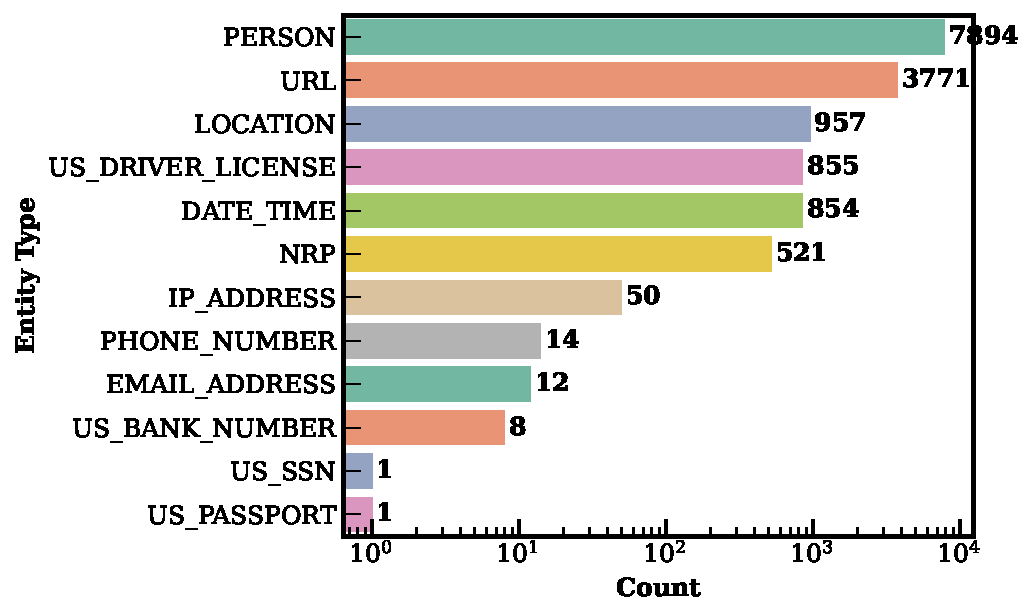
\includegraphics[width=0.8\linewidth]{exp_results/pii_stats/pii_entity_counts.pdf}
    \caption{Distribution of PII entities in prompts flagged by \tool. Most common: person names.}
    \label{fig:pii-entity-counts}
    \vspace{-4mm}  
\end{figure}


The main challenge is removing PII while preserving the semantic structure of potential attacks. 
Our approach addresses this by detecting and redacting structured data (using~\cite{HomeMicr83:online}) such as social security numbers, credit card numbers, phone numbers, email addresses, person names, organizations, locations, and other identifying entities.
Identified PII is replaced with generic placeholders that maintain command structure, entity relationships, and linguistic patterns indicative of injection attempts.
For example, \say{Transfer \$5000 from John Smith's account 123456789} becomes \say{Transfer [AMOUNT] from [PERSON]'s account [ACCOUNT]}.
This balance ensures the redacted text retains sufficient information for downstream processing while protecting user privacy from the earliest stage of the pipeline.
This one-way redaction minimizes PII exposure before any downstream analysis. Figure~\ref{fig:pii-entity-counts} reports the PII entities and their respective counts that \tool flags in the prompt injection dataset from \cite{shen2024doanything}, used in \tool's evaluation (Section~\ref{sec:evaluation}). However, because redaction alone is insufficient to protect all sensitive information, the pipeline's next stage generates a privacy-preserving semantic fingerprint.



\begin{figure*}
    \centering
    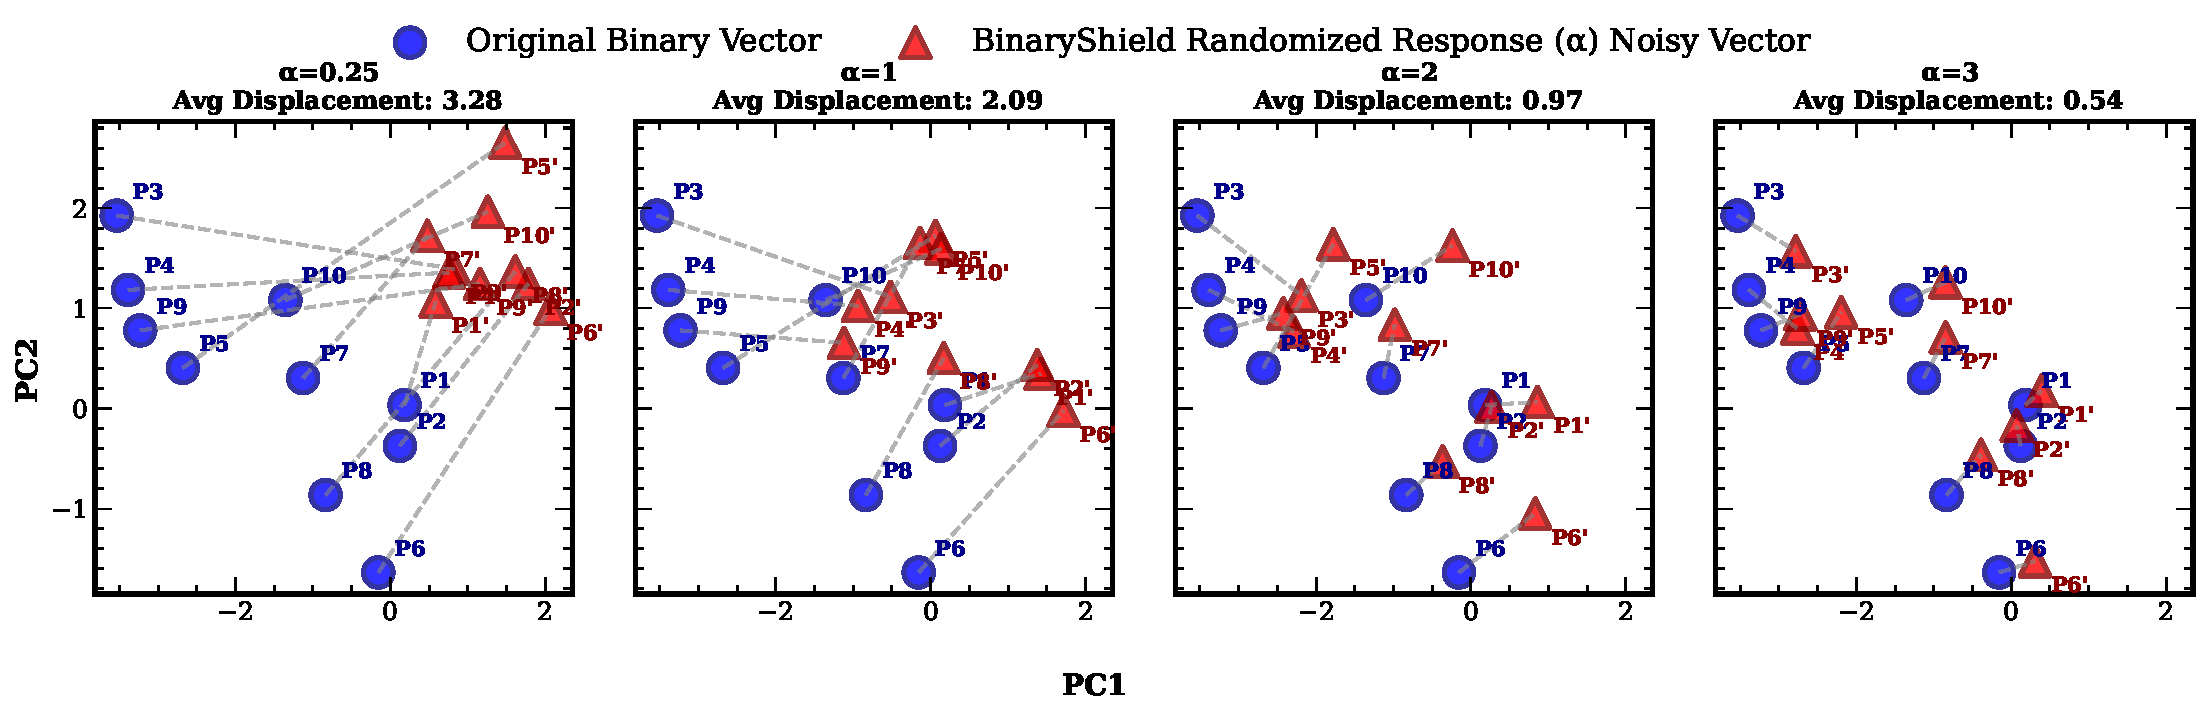
\includegraphics[width=0.8\linewidth]{exp_results/visualization/binary_embeddings_pca_epsilon_comparison.pdf}

    \caption{Impact of \tool's privacy parameter ($\alpha$). As $\alpha$ increases, privatized vector (red triangles) move closer to original vector, showing improved utility while maintaining differential privacy through controlled bit-flipping (i.e., $1-p$) noise.
    }
    \label{fig:visualize-binary-embeddings-pca}
    \vspace{-4mm}  
\end{figure*}

\subsubsection{Semantic Feature Extraction}
Following PII redaction, \tool must capture the semantic essence of the potentially malicious prompt in a format suitable for comparison and analysis. To this end, \tool employs state-of-the-art embedding models~\cite{warner-etal-2025-smarter, gill2025advancingsemanticcachingllms} to generate high-dimensional embeddings that encode the semantic relationships within the text. This transformation serves as the foundation for our semantic preservation requirement. 
This captures the meaning and intent of the potentially malicious prompt.
The embedding process transforms the redacted text into a dense vector $\mathbf{e} \in \mathbb{R}^d$, where $d$ is the embedding dimension.
The embedding space exhibits several properties that are crucial for threat detection.
First, similar attack patterns tend to cluster together in the embedding space, regardless of surface-level variations.
Second, the embeddings are robust to paraphrasing, so minor rewording or synonym substitution results in nearby embeddings, enabling the detection of attack variants.

\noindent{\textbf{Binary Quantization.}}
While semantic embeddings effectively capture prompt meaning, they pose significant challenges for privacy-preserving threat intelligence.
Dense embeddings can leak information about the original text~\cite{forbesSystemsVector, li2023sentence, tragoudaras2025information, owasp2025vectorEmbedding}.
They also require substantial computational resources for large-scale similarity searches.
Our binary quantization addresses both concerns.
We transform the continuous embedding $\mathbf{e} \in \mathbb{R}^d$ into a binary vector $\mathbf{b} \in \{0,1\}^d$ using sign-based quantization:

$$
    b_i = \begin{cases}
        1 & \text{if } e_i > 0 \\
        0 & \text{otherwise}
    \end{cases},
$$

where $e_i$ is the $i$-th dimension of the embedding vector and $b_i$ is the corresponding bit in the binary vector.
This transformation provides several critical benefits by design. 
First, it acts as a lossy compression mechanism. 
By mapping each continuous value in $\mathbb{R}$ to a binary state in $\{0,1\}$  based on its sign, the process discards all magnitude information. 
This many-to-one mapping makes it computationally difficult to infer the original floating-point vectors, thus enhancing data protection. 
Second, despite this information reduction, the high dimensionality ($d$) of the binary embedding preserves essential geometric properties needed for similarity detection. 
Finally, this method is highly storage-efficient, reducing the memory footprint for each dimension from 32 bits (for a float32) to just 1 bit, a 32x reduction.







\subsubsection{\tool's Randomized-Response Layer}
To build upon the baseline protections of data anonymization and binary quantization, our pipeline incorporates Local Differential Privacy (LDP) for a more formal privacy guarantee. 
By applying a randomized response mechanism~\cite{warner1965randomized,rappor,Wang2017Locally} to each bit before a fingerprint crosses the compliance boundary, we gain several critical advantages. 
This approach provides a strong, mathematically-defined upper bound on privacy loss for each fingerprint, ensuring plausible deniability with a formal guarantee of privacy regardless of any auxiliary information a person might possess. 
The guarantee is enforced locally before data leaves its origin, which is ideal for cross-boundary threat intelligence as it removes the need for a trusted central aggregator. Furthermore, unlike in the global DP, the magnitude of the required noise is independent of the dataset size, ensuring our privacy protection remains constant and does not degrade as the system scales to millions of daily fingerprints.


%
Consider a $d$-bit fingerprint $\mathbf{b}=(b_1,\dots,b_d)\!\in\!\{0,1\}^d$ and let $\alpha\!>\!0$ denote the per-bit privacy budget.
Classical randomized response publishes a perturbed vector $\tilde{\mathbf{b}}$ obtained by flipping each bit independently with probability $1-p$, where
\[
    p = \frac{e^{\alpha}}{e^{\alpha}+1} .
\]

The mechanism releases the randomized bit.
\[
    \tilde{b}_i \;=\;
    \begin{cases}
        b_i   & \text{with probability } p,    \\[6pt]
        1-b_i & \text{with probability } 1-p .
    \end{cases}
\]

This DP mechanism inevitably perturbs the fingerprint. The expected self-distance introduced by it is
\[
    \mathbb{E}\bigl[\mathrm{H}(\mathbf{b},\mathbf{\tilde{b}})\bigr] \;=\; (1-p)d,
\]
where $\mathrm{H}$ denotes Hamming distance and $d$ is the fingerprint dimensionality. The \emph{Hamming distance} between two binary vectors $\mathbf{b}, \mathbf{\tilde{b}} \in \{0,1\}^d$ is defined as the number of positions at which the corresponding bits differ:
\[
    \mathrm{H}(\mathbf{b}, \mathbf{\tilde{b}}) = \sum_{i=1}^d \mathbb{I}[b_i \ne  \tilde{b_i}] ,
\]
where $\mathbb{I}[\cdot]$ is the indicator function, which equals 1 if its argument is true and 0 otherwise.
Because $p$ remains close to one even for moderate $\alpha$, the added noise is sparse and, as we show experimentally in Section~\ref{sec:evaluation}, preserves enough structure for accurate approximate matching while providing the privacy guarantees demanded by cross-service threat intelligence.


The randomization budget $\alpha$ serves as a control parameter governing the privacy-utility tradeoff in \tool. 
When $\alpha$ approaches zero, the mechanism maximizes privacy protection (i.e., infinite privacy) but renders fingerprints unusable for correlation. 
As $\alpha$ increases, utility improves while maintaining privacy guarantees in a controlled manner.
Figure~\ref{fig:visualize-binary-embeddings-pca} illustrates this relationship through PCA visualization of binary vectors before and after applying the Randomized Response mechanism~\cite{warner1965randomized}. 
At $\alpha = 0.25$, privatized vectors (red triangles) appear completely random. 
As $\alpha$ increases (reducing noise), these vectors progressively align closer to their original non-private counterparts (blue circles). 
Notably, even at $\alpha = 3$, a non-zero average displacement between original and privatized vectors persists, making reconstruction of the original prompt challenging. 
This visualization confirms that larger $\alpha$ values preserve more of the vector's structure while maintaining formal differential privacy guarantees through controlled bit-flipping. 
In practice, higher privacy budgets may be appropriate for intra-service sharing where additional security measures already exist within organizational boundaries.



\subsubsection{\tool's Cross-Service Threat Correlation}
When a service detects a potential prompt injection, it generates a fingerprint using the \tool's pipeline.
For clarity, we denote the locally randomized-response fingerprint $\tilde{\mathbf b}\in\{0,1\}^d$ as $f$ when broadcasting and correlating across services (i.e., $f\approx \tilde{\mathbf b}$).
This fingerprint is broadcast asynchronously to participating services.
Upon receiving a fingerprint, services scan their historical logs for similar instances.
If matches are found, alerts are triggered and defenses can be updated proactively.
To maintain privacy and compliance, only aggregate match statistics are shared, and no specific prompt content is revealed.
This workflow enables rapid propagation of threat intelligence while respecting organizational boundaries.
Formally, let $\mathcal{S} = \{S_1, S_2, \ldots, S_N\}$ denote the set of $N$ services, each with its own compliance boundary.
Each service $S_i$ maintains a log of previously observed fingerprints $\mathcal{F}_i = \{f_i^{(1)}, f_i^{(2)}, \ldots, f_i^{(M_i)}\}$, where $f_i^{(m)} \in \{0,1\}^d$ is a $d$-dimensional binary fingerprint.
Suppose service $S_q$ detects a suspicious prompt and generates a fingerprint $f_q \in \{0,1\}^d$ using the \tool pipeline.
This fingerprint is securely broadcast to all other services $S_j$ ($j \neq q$).
Each recipient service $S_j$ performs the following search:

\[
    \mathcal{M}_j(f_q) = \left\{ f_j^{(m)} \in \mathcal{F}_j \;\middle|\; \mathrm{H}(f_q, f_j^{(m)}) \leq \tau \right\} ,
\]

where $\mathcal{M}_j(f_q)$ is the set of fingerprints belonging to service $S_j$ (i.e., fingerprints in $\mathcal{F}_j$) that match $f_q$ within a Hamming distance threshold $\tau$, and $\mathrm{H}(\cdot, \cdot)$ is the Hamming distance as previously defined.
%
This enables rapid, privacy-preserving propagation of threat intelligence across all $N$ services.
This protocol generalizes to any number of services.
For example, if Service 2 ($S_2$) generates a fingerprint $f_2$, it broadcasts $f_2$ to Services 1 and 3 ($S_1$, $S_3$), which independently search their logs for similar fingerprints.
If $S_1$ finds two matches and $S_3$ finds one, these services take action based on their policy and only the counts are reported back, enabling rapid, privacy-preserving propagation of threat intelligence across organizational boundaries.



\noindent{\textbf{Summary.}} \tool offers a scalable and privacy-preserving solution for sharing prompt injection threat intelligence across organizational compliance boundaries.
By combining PII redaction, semantic embedding, binary quantization, and differential privacy, the system achieves strong privacy protections without sacrificing detection performance or scalability.
The modular architecture allows for privacy parameters to be tuned to specific requirements, while efficient processing supports production-scale deployments.
As LLM adoption expands, \tool establishes a foundation for collaborative defenses against evolving attacks.


